\documentclass[tikz, border=0px]{standalone}
\usepackage{tikz}
\usetikzlibrary{shapes,arrows}

\tikzstyle{startstop} = [rectangle,rounded corners,minimum width=3cm,minimum height=1cm,align=center,draw=black, text width=2.5cm, fill=green!30]

\tikzstyle{therapy} = [trapezium, trapezium left angle =70, trapezium right angle=110, minimum width=2cm, minimum height = 1cm, centered,draw=black,align=center, text width=2cm, fill=orange!30]

\tikzstyle{decision} = [diamond, minimum width = 3cm, minimum height = 3cm, text centered, draw=black, text width = 2cm,align=center,fill=blue!30]

\tikzstyle{arrow} = [thick, ->, >=stealth]
\tikzstyle{doublearrow} = [<->, thick, >=stealth]

\begin{document}
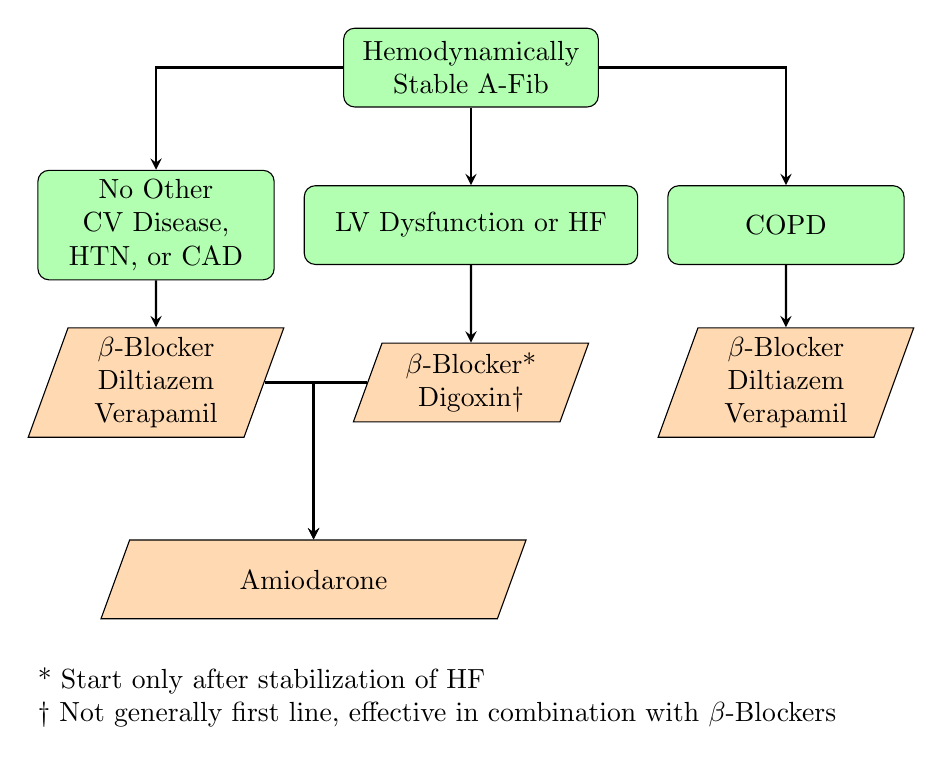
\begin{tikzpicture}[node distance=2cm]

\node (start) [startstop, text width=3cm] {Hemodynamically Stable A-Fib};
\node (healthy) [startstop, below of=start,xshift=-4cm] {No Other CV Disease, HTN, or CAD};
\node (hf) [startstop, below of=start,xshift=0cm,text width=4cm] {LV Dysfunction or HF};
\node (copd) [startstop, below of=start,xshift=4cm] {COPD};
\node (healthydrugs) [therapy, below of=healthy] {$\beta$-Blocker Diltiazem Verapamil};
\node (hfdrugs) [therapy, below of=hf] {$\beta$-Blocker* Digoxin$\dagger$};
\node (copddrugs) [therapy, below of=copd] {$\beta$-Blocker Diltiazem Verapamil};
\node (amiodarone) [therapy, below of=healthydrugs, yshift=-0.5cm, xshift=2cm] {Amiodarone};

\node (footnote) [rectangle, fill=none, below of=start, text width= 11cm, yshift=-6cm] {* Start only after stabilization of HF \\ $\dagger$ Not generally first line, effective in combination with $\beta$-Blockers};

\draw [arrow] (start) -- (hf);
\draw [arrow] (start) -| (healthy);
\draw [arrow] (start) -| (copd);
\draw [arrow] (copd) -- (copddrugs);
\draw [arrow] (healthy) -- (healthydrugs);
\draw [arrow] (hf) -- (hfdrugs);
\draw [arrow] (hfdrugs) -| (amiodarone);
\draw [arrow] (healthydrugs) -| (amiodarone);

\end{tikzpicture}
\end{document}